\section{绪论}
轨道交通全称为城市快速轨道交通,是指城市中有轨的大运量的公共交通运输系统。目前国际轨道交通地铁、轻轨、磁悬浮列车等多种类型,其中轻轨就是地面的轨道交通,其他面运行采取的是全隔离方式或者架起来,尽量不占或少占城市道路,与常规交通的平面交叉\cite{HuGuoLiang2009ANSYS}。

随着我国轨道交通的快速发展,包括城市轨道交通系统和区域城际轨道交通系统,对轨道车辆的设计提出了更高的要求,因此需要采用更加先进和合理的设计方法来完成轨道车辆整体设计。作为一种先进的设计手段,动态设计方法已经成为企业提高竞争力的重要方法。要进行动态设计,前提是对车辆的动态性能作出正确的分析\citet{ZhuQingJun2010Analysis}。

本论文主要针对轨道车辆过道门进行模态研究分析,从而为提高轨道车辆的设计水平,将现代化的设计方法应用于轨道车辆整体的设计提出合理化建议。
\subsection{课题的提出及背景}
\subsubsection{国内外车门的发展现状}
德国、奥地利和日本的铁路工业是世界的佼佼者,尤其是日本的铁路新干线开创了日本铁路产业的里程碑,也为其他国家铁路事业的发展树立了榜样。在车门的研究方面日本也有实质性的突破,尤其表现在自动关门机的开发上。他们在设计通勤电动客车时,车门没有设台阶,以便旅客能平稳流动以及安全、迅速上下车,具有缩短停车时间的显著功能\citep{ChengHeng2010Applications}。

为了缓和客流高峰、缩短上下车时间,从209系、E217系以后的“新系列车辆”起,JR东日本客运公司就在市郊型电力客车一侧设置了4个车门,并将其规定为通勤电动客车的车门设置标准。为了贯彻该自动关门机要求的“高可靠性、操纵力易于控制、减少修理”的新理念,JR东日客公司于1992年首次开发了电气式自动关门机构,并安装于901系列编组车上在京摈东北根岸线上试用。

\begin{figure}
    \centering
    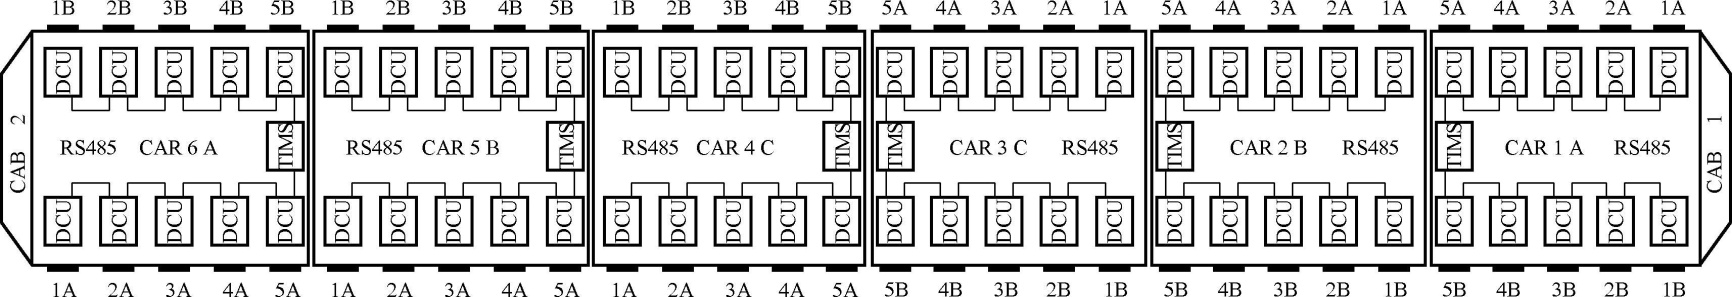
\includegraphics[width=0.8\textwidth]{trial.jpg}
    \caption{轨道车辆车门分布简图}
    \label{fig:trial}
\end{figure}

$\cdots\cdots$